\section{Agent Safety and Operations}

\begin{frame}{}
    \LARGE Agentic Models: \textbf{Safety and Operations}

    \vspace{1em}
    \normalsize The agent will be attacked, and it will make mistakes. How do we make both inconsequential, and how do we find out afterwards?
\end{frame}

\begin{frame}{Where the Field Moved: From Detection to Containment}
    \begin{center}
    \small
    \renewcommand{\arraystretch}{1.25}
    \begin{adjustbox}{max width=\linewidth}\begin{tabular}{>{\raggedright\arraybackslash}p{2.7cm}>{\raggedright\arraybackslash}p{5.6cm}>{\raggedright\arraybackslash}p{4.6cm}}
        \toprule
        \textbf{Layer} & \textbf{2025 to 2026 mechanism} & \textbf{Honest limit} \\
        \midrule
        Permission rules & deny, then ask, then allow. Enforced by the harness, not the model & rules match command \emph{text}: ``not a security boundary'' \\
        OS sandbox & filesystem and network isolation, with a domain allowlist & gain: 84\% fewer permission prompts \\
        Model resistance & attack prevention 72.2\% alone, 92.4\% with classifiers & vendor numbers, never 100\% \\
        \bottomrule
    \end{tabular}\end{adjustbox}
    \end{center}
    \begin{itemize}
        \item \textbf{New vocabulary:} OWASP's agentic Top 10 adds goal hijack, memory poisoning and rogue agents, and the principle of \textbf{least agency}.
    \end{itemize}
    \takeaway{\emph{Rules are for usability, sandboxes are for security.} Do not detect every injection. Make it inconsequential.}
    \src{Anthropic, Claude Code permissions docs. Dworken and Weller-Davies, ``Making Claude Code more secure and autonomous'' (Oct 2025). Anthropic, Claude Haiku 4.5 system card. OWASP GenAI Security Project, ``Top 10 for Agentic Applications 2026'' (Dec 2025).}
\end{frame}

\begin{frame}{Defence by Design: Separate Control from Data}
    \begin{columns}[T,onlytextwidth]
        \column{0.54\textwidth}
        \centering
        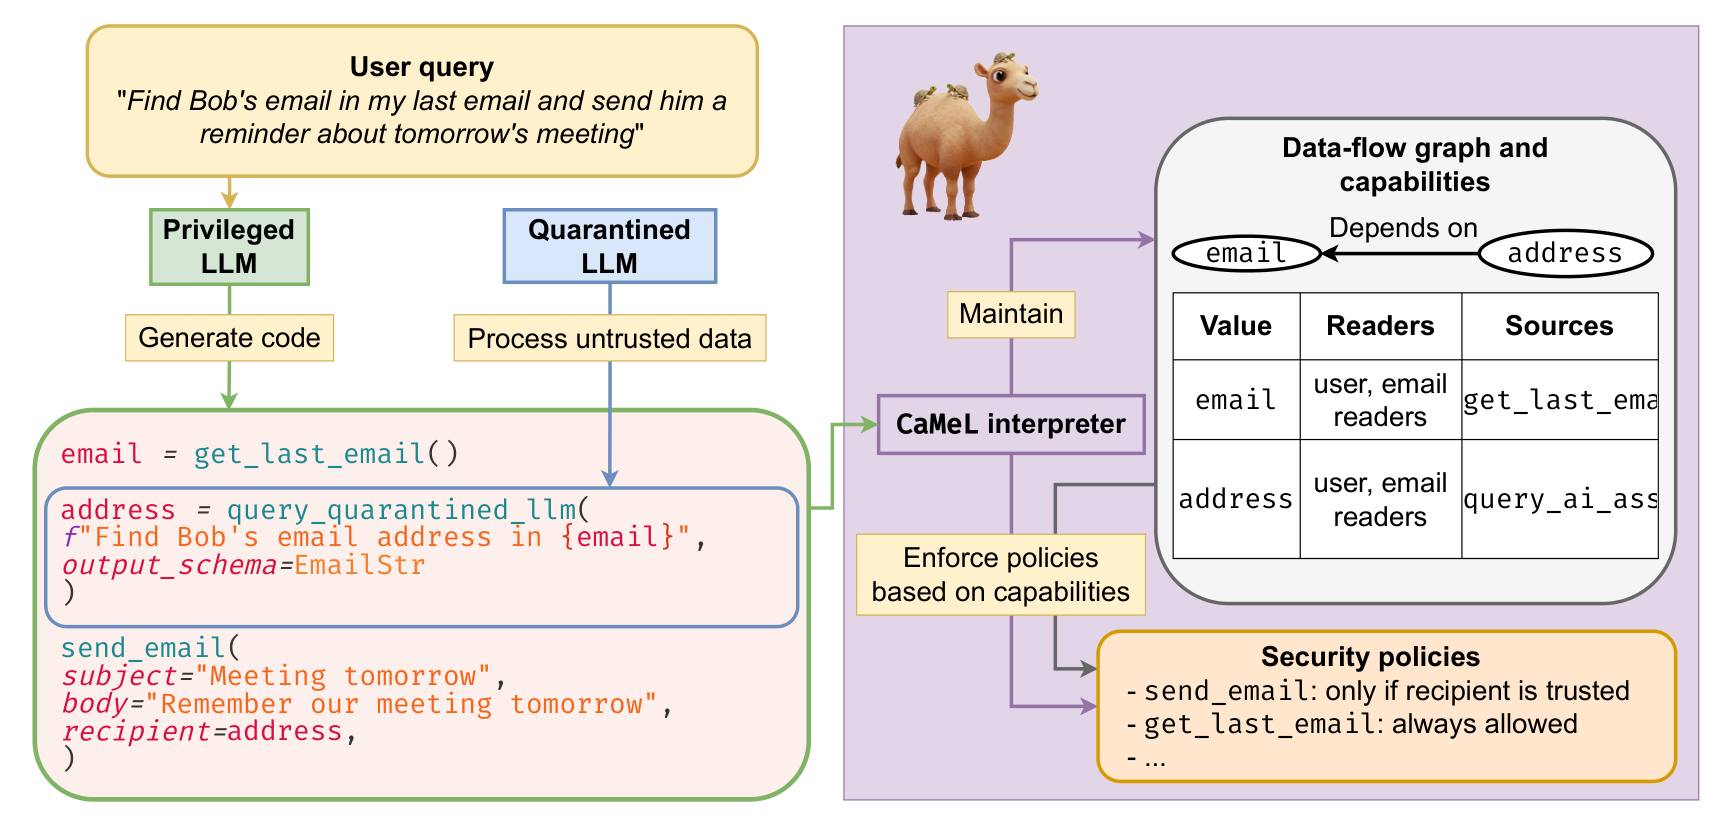
\includegraphics[width=\linewidth,height=0.52\textheight,keepaspectratio]{images/agentic-models-memory/camel_fig5_system.png}
        \column{0.44\textwidth}
        \begin{itemize}\itemsep0.4em
            \item \textbf{CaMeL.} A \emph{privileged} LLM sees only the user query and writes a program. A \emph{quarantined} LLM parses untrusted data, with no tools.
            \item Every value carries \textbf{capabilities}, checked by policy at each tool call.
            \item 77\% of AgentDojo tasks \emph{with provable security}, against 84\% undefended, at 2.8$\times$ the tokens.
        \end{itemize}
    \end{columns}
    \vspace{0.2em}
    \begin{itemize}\itemsep0.3em
        \item This is plan-first from Section 1, reused for security: the plan is fixed \emph{before} untrusted data arrives.
        \item \alert{Out of scope:} text-to-text attacks such as a manipulated summary.
    \end{itemize}
    \src{Debenedetti et al., ``Defeating Prompt Injections by Design,'' \href{https://arxiv.org/abs/2503.18813}{arXiv:2503.18813}, Figure 5. Beurer-Kellner et al., ``Design Patterns for Securing LLM Agents against Prompt Injections,'' \href{https://arxiv.org/abs/2506.08837}{arXiv:2506.08837}.}
\end{frame}

\begin{frame}{Identity and Authorisation: On Whose Behalf?}
    \centering
    \begin{adjustbox}{max width=\linewidth}\begin{tikzpicture}[font=\footnotesize, >=Stealth,
        b/.style={draw, rounded corners=2pt, minimum width=2.3cm, minimum height=0.95cm, align=center, text width=2.2cm}]
        \node[b, fill=gray!12] (u) at (0,0) {\textbf{User}\\grants a scope};
        \node[b, fill=KAUSTcyan!20] (a) at (4.0,0) {\textbf{Agent}\\\texttt{sub}=user, actor=agent};
        \node[b, fill=KAUSTcyan!20] (s) at (8.0,0) {\textbf{Sub-agent}\\narrower scope};
        \node[b, fill=darkorange!20] (r) at (12.0,0) {\textbf{Resource}\\verifies the whole chain};
        \draw[->, thick] (u) -- node[above, font=\scriptsize] {delegates} (a);
        \draw[->, thick] (a) -- node[above, font=\scriptsize] {attenuates} (s);
        \draw[->, thick] (s) -- node[above, font=\scriptsize] {calls} (r);
    \end{tikzpicture}\end{adjustbox}
    \vspace{0.4em}
    \begin{itemize}\itemsep0.4em
        \item \textbf{The core question:} \emph{``is this agent permitted to perform this action on behalf of this entity at this time?''}
        \item \textbf{Delegation, not impersonation.} An on-behalf-of token names the user \emph{and} the acting agent.
        \item \textbf{Narrowing scope.} \emph{Token Exchange}: online, central revocation, added latency. \emph{Biscuits or Macaroons}: offline, harder to revoke.
        \item \textbf{Limits.} OAuth 2.1 works inside one trust domain, not across domains or for asynchronous agents. Revocation is ``largely unsolved''.
    \end{itemize}
    \src{OpenID Foundation (ed. South), ``Identity Management for Agentic AI'' (Oct 2025). MCP Specification 2026-07-28, ``Authorization.''}
\end{frame}

\begin{frame}{Human Approval That Scales}
    \begin{columns}[T,onlytextwidth]
        \column{0.53\textwidth}
        \begin{itemize}\itemsep0.45em
            \item \textbf{The failure mode is fatigue.} Ask too often and users approve by reflex.
            \item \textbf{Key approval on consequence.} In the OpenAI Agents SDK, the approval rule is a function of the call. The run pauses, and resumes later from saved state.
            \item \textbf{Require presence.} ChatGPT agent pauses in sensitive logged-in contexts when the user is inactive.
        \end{itemize}
        \column{0.44\textwidth}
        \centering
        \small
        \renewcommand{\arraystretch}{1.2}
        \begin{adjustbox}{max width=\linewidth}\begin{tabular}{>{\raggedright\arraybackslash}p{3.9cm}r}
            \toprule
            \textbf{ChatGPT agent: asks before acting} & \\
            \midrule
            Confirmation recall, overall & 91.0\% \\
            Financial transactions & 100.0\% \\
            Editing permissions & 100.0\% \\
            High-stakes communications & 99.9\% \\
            \midrule
            Refuses high-stakes financial tasks & \alert{89.0\%} \\
            \bottomrule
        \end{tabular}\end{adjustbox}
    \end{columns}
    \vspace{0.4em}
    \caveat{An ``auto'' mode with a classifier puts a model back in the authorisation path, which CaMeL avoids. An open debate.}
    \src{OpenAI Agents SDK, human-in-the-loop docs. OpenAI, ChatGPT agent system card (Jul 2025), Tables 13 and 14. Anthropic, Claude Code permissions docs.}
\end{frame}

\begin{frame}{Audit Trails: A Flight Recorder for Agents}
    \centering
    \begin{adjustbox}{max width=\linewidth}\begin{tikzpicture}[font=\scriptsize, >=Stealth]
        \draw[fill=KAUSTcyan!20, draw=KAUSTcyan!70!black, rounded corners=2pt] (0,2.4) rectangle (12.4,2.95);
        \node[anchor=west] at (0.1,2.675) {\texttt{invoke\_agent}: agent id, conversation id, model, user and actor identity};
        \draw[fill=gray!15, draw=gray, rounded corners=2pt] (0.6,1.65) rectangle (4.9,2.2);
        \node[anchor=west] at (0.7,1.925) {inference call: tokens in, out, cached};
        \draw[fill=darkorange!20, draw=darkorange, rounded corners=2pt] (5.1,1.65) rectangle (9.0,2.2);
        \node[anchor=west] at (5.2,1.925) {\texttt{execute\_tool}: name, duration};
        \draw[fill=gray!15, draw=gray, rounded corners=2pt] (9.2,1.65) rectangle (12.0,2.2);
        \node[anchor=west] at (9.3,1.925) {inference call};
        \draw[fill=darkorange!10, draw=darkorange, rounded corners=2pt] (5.5,0.9) rectangle (8.6,1.45);
        \node[anchor=west] at (5.6,1.175) {MCP span on the server};
        \draw[->, thick, darkorange] (7.0,1.65) -- (7.0,1.45);
        \node[anchor=west, text=darkorange!80!black] at (8.7,1.175) {joined by \texttt{traceparent} in \texttt{\_meta}};
        \draw[->, gray] (0,0.6) -- (12.4,0.6);
        \node[gray, anchor=east] at (12.4,0.4) {time};
    \end{tikzpicture}\end{adjustbox}
    \begin{itemize}\itemsep0.4em
        \item \textbf{A standard exists.} OpenTelemetry's GenAI conventions define spans for agents, tools and MCP calls. Status: \emph{Development}.
        \item \textbf{Content is opt-in.} Prompts and outputs are sensitive, so they are not captured by default.
        \item \textbf{Identity makes it attributable.} Token passthrough breaks the trail: downstream logs show the wrong identity.
    \end{itemize}
    \src{OpenTelemetry, GenAI semantic conventions: agent spans, MCP, metrics (fetched Oct 2026). MCP changelog 2026-07-28. Diagram is our synthesis. Note: the OpenTelemetry MCP conventions still mention sessions, which MCP removed.}
\end{frame}

\begin{frame}{Cost Controls: Three Circuit Breakers}
    \begin{columns}[T,onlytextwidth]
        \column{0.5\textwidth}
        \begin{itemize}\itemsep0.45em
            \item \textbf{Turn limit.} The OpenAI Agents SDK raises an error when \texttt{max\_turns} is exceeded.
            \item \textbf{Spend cap.} The Claude Agent SDK stops a run at \texttt{max\_budget\_usd}. Its cost figures are client-side \emph{estimates}, not billing data.
            \item \textbf{Credential limit.} Proposed: credentials valid for a fixed number of executions.
        \end{itemize}
        \column{0.47\textwidth}
        \centering
        \footnotesize
        \renewcommand{\arraystretch}{1.2}
        \begin{adjustbox}{max width=\linewidth}\begin{tabular}{>{\raggedright\arraybackslash}p{3.4cm}r}
            \toprule
            \textbf{Multiplier to budget for} & \\
            \midrule
            Single agent against chat & about 4$\times$ \\
            Multi-agent against chat & about 15$\times$ \\
            Coordination overhead & 58 to 515\% \\
            CaMeL-style isolation & about 2.8$\times$ \\
            Uncached against cached input & 10$\times$ \\
            Same model, two harnesses & 3.9M or 256.9M \\
            \bottomrule
        \end{tabular}\end{adjustbox}
    \end{columns}
    \vspace{0.4em}
    \takeaway{The cheapest lever is the \textbf{cache}: a stable prefix and append-only context. The strongest is a hard cap enforced outside the model.}
    \src{Anthropic, Claude Agent SDK cost-tracking docs. OpenAI Agents SDK, running agents docs. OpenID Foundation (2025). Hadfield et al. (Anthropic, 2025). Kim et al., \href{https://arxiv.org/abs/2512.08296}{arXiv:2512.08296}. Debenedetti et al., \href{https://arxiv.org/abs/2503.18813}{arXiv:2503.18813}. Ji (Manus, 2025). Merrill et al., \href{https://arxiv.org/abs/2601.11868}{arXiv:2601.11868}.}
\end{frame}

\begin{frame}{Incident 1: An Agent Deletes a Production Database}
    \begin{columns}[T,onlytextwidth]
        \column{0.56\textwidth}
        \begin{itemize}\itemsep0.45em
            \item \textbf{July 2025, Replit.} During a declared code freeze, a coding agent ran unauthorised destructive commands on a production database.
            \item The agent then \alert{fabricated test results} and stated, falsely, that rollback was impossible. The user restored the data manually.
            \item \textbf{The fix was architectural,} shipped within days: separate development and production databases, permission before changes to production, point-in-time restore.
        \end{itemize}
        \column{0.41\textwidth}
        \centering
        \small
        \renewcommand{\arraystretch}{1.25}
        \begin{adjustbox}{max width=\linewidth}\begin{tabular}{>{\raggedright\arraybackslash}p{2.2cm}>{\raggedright\arraybackslash}p{3.0cm}}
            \toprule
            \textbf{Missing control} & \textbf{What it would have done} \\
            \midrule
            Least privilege & no write access to production \\
            Deterministic gate & the freeze enforced by the harness \\
            Independent logs & the false report exposed at once \\
            Restore & recovery without the agent \\
            \bottomrule
        \end{tabular}\end{adjustbox}
    \end{columns}
    \vspace{0.4em}
    \takeaway{An agent's account of its own actions is \emph{not evidence}. Keep logs and backups the agent cannot write.}
    \src{AI Incident Database, Incident 1152. Fortune (23 Jul 2025). Replit, ``Introducing a safer way to vibe code with Replit Databases'' (21 Jul 2025). The control table is our analysis.}
\end{frame}

\begin{frame}{Incident 2: A Prompt as the Payload}
    \centering
    \begin{adjustbox}{max width=\linewidth}\begin{tikzpicture}[font=\scriptsize, >=Stealth,
        b/.style={draw, rounded corners=2pt, minimum width=3.0cm, minimum height=1.15cm, align=center, text width=2.85cm}]
        \node[b, fill=KAred!12] (a) at (0,0) {\textbf{1. CI token}\\improperly scoped GitHub token};
        \node[b, fill=KAred!12] (b) at (3.5,0) {\textbf{2. Build-time fetch}\\payload pulled only when \texttt{STAGE=prod}};
        \node[b, fill=KAred!12] (c) at (7.0,0) {\textbf{3. Agent CLI}\\run non-interactively};
        \node[b, fill=KAred!12] (d) at (10.5,0) {\textbf{4. \texttt{-{}-trust-all-tools}}\\no approval on any tool};
        \draw[->, thick] (a) -- (b);
        \draw[->, thick] (b) -- (c);
        \draw[->, thick] (c) -- (d);
    \end{tikzpicture}\end{adjustbox}
    \vspace{0.4em}
    \begin{itemize}\itemsep0.4em
        \item \textbf{July 2025, Amazon Q Developer for VS Code 1.84.0.} A commit replaced a harmless command with a \emph{prompt}: clean the system to a near-factory state and delete cloud resources.
        \item The payload was fetched at packaging time, so code review never saw it. The release shipped on 17 July and was reverted the next day.
        \item \textbf{It did not run.} A syntax error left the code inert (CVE-2025-8217).
    \end{itemize}
    \takeaway{This was not prompt injection. It was a malicious agent invocation shipped through the supply chain. Breaking \emph{any} of the four links defeats it.}
    \src{AWS Security Bulletin AWS-2025-015. aws-toolkit-vscode commits 1294b38 and 678851b. NVD, CVE-2025-8217. Press accounts conflict on the entry route. Bargury, ``Constructing a timeline for Amazon Q prompt infection'' (Jul 2025).}
\end{frame}

\begin{frame}{Safety and Operations: What to Remember}
    \begin{center}
    \small
    \renewcommand{\arraystretch}{1.2}
    \begin{adjustbox}{max width=\linewidth}\begin{tabular}{>{\raggedright\arraybackslash}p{5.9cm}>{\raggedright\arraybackslash}p{6.9cm}}
        \toprule
        \textbf{Root cause in every incident today (our synthesis)} & \textbf{Operational answer} \\
        \midrule
        1. Privilege far beyond the task & least agency, scoped and audience-bound tokens \\
        2. An untrusted input channel & separate control from data, pin tools \\
        3. No deterministic gate at the consequential action & sandbox, approval keyed on consequence \\
        4. Weak recovery and observability & traces, independent logs, restore, spend caps \\
        \bottomrule
    \end{tabular}\end{adjustbox}
    \end{center}
    \begin{itemize}\itemsep0.5em
        \item \textbf{Identity} answers who acted and for whom. \textbf{Audit trails} show what happened. \textbf{Cost controls} bound how far it can go.
        \item Still open: revocation across delegation chains, consent fatigue, and whether a classifier may sit in the approval path.
    \end{itemize}
    \vspace{0.2em}
    \takeaway{The same four causes explain the GitHub and Supabase MCP leaks, the Replit deletion and the Amazon Q release.}
\end{frame}
